\documentclass{article}
\usepackage{graphicx}
\graphicspath{ {images/} }


\newcommand{\tab}[1]{\hspace{.1\textwidth}\rlap{#1}}

\begin{document}
	
\begin{titlepage}
	\newcommand{\HRule}{\rule{\linewidth}{0.5mm}} % Defines a new command for the horizontal lines, change thickness here

	\center % Center everything on the page
	 
	%----------------------------------------------------------------------------------------
	%	LOGO SECTIONS
	%----------------------------------------------------------------------------------------

	\includegraphics[width=\textwidth]{front-page}

	%----------------------------------------------------------------------------------------
	%	TITLE SECTION
	%----------------------------------------------------------------------------------------

	\HRule \\[0.4cm]
	{ \huge \bfseries Software Requirements Specification}\\[0.4cm] % Title of your document
	\HRule \\[1.5cm]
	 
	%----------------------------------------------------------------------------------------
	%	MEMBERS, TEAM NAME SECTION
	%----------------------------------------------------------------------------------------

	\begin{minipage}{0.5\textwidth}
	\begin{flushleft} \large
	\emph{Members:}\\% add your name and student here
	Peter Boxall 14056136	
	
	Orisha Orrie 13025199
	
	Nsovo Baloyi 12163262
	
	Elizabeth Bode 14310156
		
	Robert Trankle 15092454

	Nikki Constancon 15011713

	Ernst Eksteen 28398603
	\end{flushleft}
	\end{minipage}
	~
	\begin{minipage}{0.4\textwidth}
	\begin{flushright} \large
	{ \huge \bfseries Team Fuchsia }% Title of document
	{\large \today}\\
	{\large v0.1}
	\end{flushright}
	\end{minipage}\\[4cm]
\end{titlepage}


	\newpage
	
	\section{Introduction}
    	
        \subsection{Purpose}
        	\paragraph{The purpose of this document is to put forth a description detailing the NavUP system. It will explain the main purpose of the system, as well as additional subsystems, the interface of these systems, and what they will and will not do, as well as the constraints. Providing a detailed requirement specification of the system as a whole. It is intended for the Client, as well as developers who will integrate the system.}
    	\subsection{Scope}
        	\paragraph{NavUP is a mobile device application, that will provide the basic functionalities of a navigation system. The system will only interoperate and function on the Hatfield main campus of the University of Pretoria.
        	
        	NavUp will provide a means to navigate the main campus of the University of Pretoria. It will thus provide users choices with regards to which routes they wish to take to reach there destination, taking into account factors such as pedestrian and vehicle traffic as well as providing routes that cater to users who may suffer physical disabilities.
        	
        	NavUP's goal is to provide a personalised, efficient and convenient means of traversing the university's Hatfield campus. The system will also provide extra additional information regarding useful points of interests such as bathroom locations, as well as provide information to the user regarding the rich history of the University of Pretoria.
        	
        	The navigation system is required to constantly be connected the the campus's WI-FI and will continually send up and down stream information to a server with regards to users location and destination. The server will be required to calculate the route and factor in additional information as set up by the user and there needs. The server must also be able to handle a high volume of concurrent users and provide them all with there required data.
        	
        	Location tracking will be achieved through the use of --WI-FI signal strength and other : not sure of exact methodology-- techniques and not through the use of GPS. /* This means that the two way communication between the device and the server must --explain requirements here-- */ }
        \subsection{Definitions, Acronyms, and Abbreviations}
        \subsection{References}
        \subsection{Overview}
	
	\section{Overall Description}
		
        \subsection{Product Perspective}
        
        	\subsubsection{System Interface}
            \subsubsection{User Interface}            
            \subsubsection{Hardware Interface}
            \subsubsection{Software Interface}
            \subsubsection{Communications Interface}
            \subsubsection{Memory}
            \subsubsection{Operations}
            	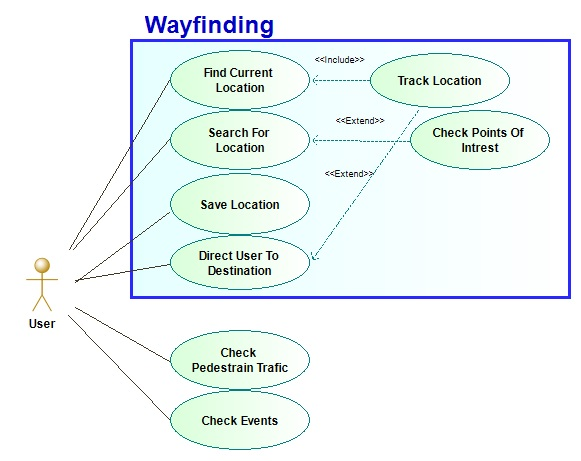
\includegraphics[scale=1]{images/COS301_Operations_Modes_a.jpg} 
            	\paragraph{The user will require a series of normal and special case operations to be fulfilled by the system. The user will use the system in normal case operations comprising of finding the users location, finding a location the user is interested in, including locations such as toilets, and navigating, tracking and guiding the user to various locations. The user will also use the system to save locations of interest for future use as well as check testicles for improved path finding, such as pedestrian traffic, vehicle traffic.
            	
            	Special modes of operation will involve the system pushing user specific information to the user device that may interest them or might require a route recalculation by the system due to environmental changes, such as pedestrian traffic flow.
            	
            	The user will primarily use the system in en-route to various locations. This will primarily take place between periods of the University time table. Other periods will primarily see the system being used by students with an off period or by visitors and lecturers. The system will see unattended periods of operations while a user is actually walking and being tracked by the system. Further unattended periods of operations will occur when the Server pushes relevant data regarding events and user preferences to the user device.
            	
            	--Data processing support functions--
            	
            	The user will be able to set there preferences and data locally on their device, but will be able to backup the data if they create a account on the system.
            	
            	--server backup??--}
            \subsubsection{Sit Adaption Requirements}
        
		\subsection{Product Functions}
    	\subsection{User Characteristics}    
    	\subsection{Constraints}   
    	\subsection{Assumptions and Dependencies}

	\section{Specific Requirements}
    
    	\subsection{External Interface Requirements}
    	\subsection{Functional Requirements}
        \subsection{Performance Requirements}
        \subsection{Design Constraints}
        \subsection{Software System Attributes}
        \subsection{Other Requirements}
	
	\section{Vision}


	\section{Background}
	
\end{document}
